
In this chapter, we will give a short overview on the basic theory of Elliptic Curves.
However, since the details are mostly the theory of algebraic geometry and do not bear too much on the main content of our work, we will keep it brief and refer the reader to the excellent textbook \cite{arithmetic_elliptic_curves}.

\section{Elliptic Curves and the group law}
Consider a field $k$ with algebraic closure $\bar{k}$.
An \emph{Elliptic Curve} is a nonsingular projective curve of genus 1 together with a special point $\IdPoint$.
If the characteristic of $k$ is not 2 or 3, each Elliptic Curve $E$ is isomorphic to a projective plane curve given by an affine equation of the form
\begin{equation*}
    E: y^2 = x^3 + Ax + B
\end{equation*}
such that the special point is the projective point at infinity $\IdPoint = (0 : 1 : 1)$ \cite[Prop.~III.3.1]{arithmetic_elliptic_curves}.
Furthermore, an isomorphism class of Elliptic Curves is uniquely determined by its j-invariant \cite[Prop.~III.1.4]{arithmetic_elliptic_curves}, defined as
\begin{equation*}
    j(E) := -1728 \frac {(4A)^3} {-16(4A^3 + 27B^3)}
\end{equation*}
Since isomorphic curves have the same properties in all aspects that matter for this work, we will use the terms Elliptic Curves and isomorphism classes of Elliptic Curves interchangeably from now on.
In particular, note that whenever we count Elliptic Curves with special properties, we only count isomorphism classes. 

The reason that makes Elliptic Curves so important is that they are abelian varieties, i.e. become groups in a way compatible with the geometric structure.
There are different characterizations of this group law, the most explicit being its representation by polynomials.
More concretely, if the curve is given by an affine equation $y^2 = x^3 + Ax + B$, then the sum of two affine points $P = (x_1 : y_1 : 1)$ and $Q = (x_2 : y_2 : 1)$ is given as
\begin{equation*}
    P + Q = ( \lambda^2\mu - x_1\mu^3 - x_2\mu^3 : \lambda(2x_1\mu^2 + x_2\mu^2 - \lambda^2) - y_1\mu^3 : \mu^3 )
\end{equation*}
where
\begin{equation*}
    (\lambda : \mu) = \begin{cases}
        (y_2 - y_1 : x_2 - x_1) & \text{if $x_1 \neq x_2$} \\
        (3x_1^2 + A : 2y_1) & \text{if $x_1 = x_2$}
    \end{cases}
\end{equation*}
Moreover, we declare the special point $\IdPoint$ to be the identity element of the group.
The nontrivial result is now that this defines a group law on the set of points of $E$ \cite[Prop.~III.2.2]{arithmetic_elliptic_curves}. 
A more theoretical characterization of the group law is given by \cite[Prop.~III.3.4]{arithmetic_elliptic_curves}, which states that the above operation $+$ is the same as the group law induced by a natural isomorphism $E \cong \mathrm{Pic}(E)$ from the points of $E$ to its Picard group. 

The two most important subgroups of the group $E$ are now the $n$-torsion group
\begin{equation*}
    E[n] := \{ P \in E \ | \ \underbrace{P + ... + P}_{\text{$n$ times}} = \IdPoint \}
\end{equation*}
and the subgroup of $k$-rational points
\begin{equation*}
    E(k) := \{ P \in E \ | \ \text{$P = (x : y : z)$ for some $x, y, z \in k$} \}
\end{equation*}

A property of Elliptic Curves that can be used for some slightly exotic cryptographic primitives (like identity-based crypto, or the verifiable delay function we present in Section~\ref{sec:verifiable_delay_function}) is the Weil pairing.
Let $m \geq 2$ be an integer coprime to $p$.
Then there exists a map, the $m$-th \emph{Weil pairing}
\begin{equation*}
    e_m: E[m] \times E[m] \to \mu_m
\end{equation*}
where $\mu_m \subseteq \C^*$ is the group of $m$-th roots of unity.
It has the following properties (see \cite[Prop.~III.8.1]{arithmetic_elliptic_curves}):
\begin{itemize}
    \item $e_m$ is bilinear, i.e. $e_m(S + S', T) = e_m(S, T)e_m(S', T)$ and similar for the second argument.
    \item $e_m$ is alternating, i.e. $e_m(T, T) = 1$.
    \item $e_m$ is nondegenerate, i.e. if $e_m(S, \cdot)$ is the constant map $\IdPoint$, then $S = \IdPoint$.
\end{itemize}

\section{Isogenies}
An \emph{isogeny} between two Elliptic Curves $E$ and $E'$ is a morphism (in the sense of algebraic geometry) that maps $\IdPoint$ to $\IdPoint$.
The first important result is that an isogeny is automatically a group homomorphism \cite[Thm~III.4.8]{arithmetic_elliptic_curves}.
The simplest example of an isogeny is the multiplication-by-$m$ map on an Elliptic Curve $E$
\begin{equation*}
    [m]: E \to E, \quad P \mapsto \underbrace{P + ... + P}_{\text{$m$ times}}
\end{equation*}

An isogeny $\psi: E \to E'$ is closely connected to the field extension $k[E]/\psi_*k[E']$, where $\psi_*: k[E'] \to k[E]$ is the associated map of $k$-algebras.
The degree of $\psi$ is then given by the degree of this field extension (it is always finite), and $\psi$ is said to be separable, if $k[E]/\psi_*k[E']$ is.
Similarly, we can define the separability degree of an isogeny.
It is a fact of algebraic geometry that both degree and separability degree behave multiplicatively under composition.
Furthermore, the separability degree of an isogeny is equal to the size of its kernel \cite[Thm~III.4.10]{arithmetic_elliptic_curves}.
It is common to call isogenies of degree $m$ also $m$-isogenies.

Studying again the example of the multiplication-by-$m$ isogeny $[m]: E \to E$, one can show that this has degree $m^2$.
Its kernel is obviously the subgroup $E[m]$, and thus, if $[m]$ is separable, we see that $E[m] \cong (\Z/m\Z)^2$.
We will explain what happens in the case that $[m]$ is inseparable in the next section.

A very important result on isogenies is that they can be classified by their kernel $\ker(\psi) \subseteq E$, which is always a finite group.
More concretely, up to isomorphism, there is a one to one correspondence
\begin{align*}
    \{ \text{Pairs $(\psi, E')$ where $\psi: E \to E'$ is a separable isogeny} \}  \ &\to \ \{ \text{Finite subgroups $G \leq E$} \} \\
    (E', \psi) \ &\mapsto \ \ker(\psi)
\end{align*}
In particular, for a finite subgroup $G \leq E$ there is a unique (up to isomorphism) Elliptic Curve $E'$ and separable isogeny $\psi: E \to E'$ with kernel $G$.
We also denote $E'$ by $E/G$, as that is the group structure on $E'$ by the isomorphism theorem (morphisms of projective irreducible curves are always surjective).

Furthermore, this correspondence is compatible with the inclusion of finite subgroups as follows.
If $G_1 \leq G_2 \leq E$ are two finite subgroups, then the unique separable isogeny $\psi: E \to E/G_2$ with kernel $G_2$ factors through the isogeny $\phi: E \to E/G_1$, i.e. there is an isogeny $\rho: E/G_1 \to E/G_2$ with
\begin{center}
    \begin{tikzpicture}
        \node (E0) at (-4, 0) {$E$};
        \node (E1) at (0, 0) {$E/G_1$};
        \node (E2) at (4, 0) {$E/G_2$};

        \draw [->] (E0) -- (E1) node [midway, above] {$\phi$};
        \draw [->] (E1) -- (E2) node [midway, above] {$\rho$};
        \draw [->] (E0) to [bend left] node [midway, above] {$\psi$} (E2);
    \end{tikzpicture}
\end{center}
is commutative.
An analogous statement also holds for inseparable isogenies.
If $\mathrm{char}(k) = p$, then an inseparable isogeny $\psi: E \to E'$ always factors through the $p$-th power Frobenius $\pi: E \to E^{(p)}$ (which is of course purely inseparable), where $E^{(p)}$ is the Elliptic Curve with all coefficients of the defining equation raised to the $p$-th power.
Note that can also define operation $\cdot^{(p)}$ on isogenies, by again raising each coefficient in the defining polynomials to the $p$-th power.
This way, $\cdot^{(p)}$ becomes an endofunctor on the category of Elliptic Curves over $\bar{\F}_p$ and their isogenies.

The final notion we require in this context is the one of the dual isogeny.
Since the kernel of an isogeny $\psi: E \to E'$ is a subgroup of size $\deg_s(\psi)$, we see that it is contained in $E[\deg(\psi)] = \ker[\deg(\psi)]$.
Now the previous correspondence shows that $\psi$ factors through through the multiplication map $[\deg(\psi)]$, via an isogeny $\hat{\psi}$
\begin{center}
    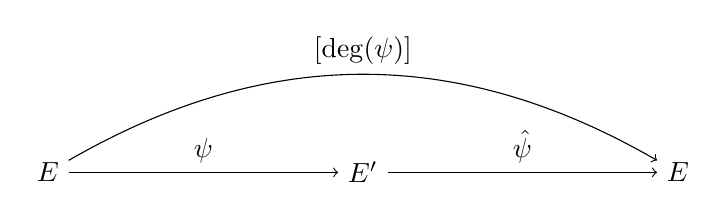
\begin{tikzpicture}
        \node (E0) at (-4, 0) {$E$};
        \node (E1) at (0, 0) {$E'$};
        \node (E2) at (4, 0) {$E$};

        \draw [->] (E0) -- (E1) node [midway, above] {$\psi$};
        \draw [->] (E1) -- (E2) node [midway, above] {$\hat{\psi}$};
        \draw [->] (E0) to [bend left] node [midway, above] {$[\deg(\psi)]$} (E2);
    \end{tikzpicture}
\end{center}
The isogeny $\hat{\psi}: E' \to E$ has then the same degree as $\psi$, and is called the \emph{dual isogeny} of $\psi$.

Interestingly, the dual isogeny behaves like an adjoint w.r.t. the Weil pairing, i.e.
\begin{equation*}
    e_m(S, \phi(T)) = e_m(\hat{\phi}(S), T)
\end{equation*}
for an isogeny $\phi: E \to E'$ and the $m$-th Weil pairing $e_m$ of $E$ resp. $E'$ (see \cite[Prop.~III.8.2]{arithmetic_elliptic_curves}).

\section{The endomorphism ring}
For an Elliptic Curve $E$, we write from now on $\End(E)$ for the set of isogenies $E \to E$.
Via composition and pointwise addition, this becomes a (possibly noncommutative) unital ring.
The existence of the multiplication-by-$m$ isogeny implies that there is a ring homomorphism
\begin{equation*}
    \Z \to \End(E)
\end{equation*}
As it turns out, this is always injective \cite[Prop.~III.4.2]{arithmetic_elliptic_curves}, hence the endomorphism ring has characteristic 0.
Much more is known about the endomorphism ring, though.
In particular, there is the following theorem
\begin{theorem}
    Let $E$ be an Elliptic Curve over $k$. Then $\End(E)$ is one of the following
    \begin{itemize}
        \item The ring of integers $\Z$.
        \item An order in a quadratic imaginary number field.
        \item An order in the quaternion algebra ramified exactly at $p$ and $\infty$, where $p = \mathrm{char}(k)$.
    \end{itemize}
    If $\mathrm{char}(k) = 0$, only the first two are possible.
    Similarly, if $\mathrm{char}(k) \neq 0$, only the last two are possible. 
\end{theorem}
For a proof, see e.g. \cite[Corollary~III.9.4]{arithmetic_elliptic_curves}.

If $\mathrm{char}(k) \subseteq \bar{\F}_p$, we call the curve $E$ \emph{ordinary} in the second case and \emph{supersingular} in the third case.
There are some other fundamental differences between those two types, as displayed in the following table.
Denote by $\pi_E$ the $q$-th power Frobenius, where $E$ is defined over $\F_q$.
\begin{center}
    \begin{tabular}{c | c}
        ordinary & supersingular \\
        \hline
        $[p]$ has separability degree $p$ & $[p]$ is totally inseparable \\
        $E[p] \cong \Z/p\Z$ & $E[p] = \{ \IdPoint \}$ \\
        $\End(E)$ is commutative & $\End(E)$ is not commutative \\
        $\mathrm{Tr}(\pi_E) \not\equiv 0 \mod p$ & $\mathrm{Tr}(\pi_E) \equiv 0 \mod p$ \\
        $\hat{\pi}_E$ separable & $\hat{\pi}_E$ totally inseparable \\
        $p \notdivides d(\End(E))$ and $p \notdivides d(\Z[\pi_E])$ & $p \divides d(\Z[\pi_E])$
    \end{tabular}
\end{center}
Note that the trace
\footnote{By trace, we mean either the trace in the quadratic imaginary number field, or the reduced trace in the quaternion algebra. In particular, if $\pi_E = \pm p$ (the supersingular setting with $E/\F_{p^2}$), we have $\mathrm{Tr}(\pi_E) = \pm 2p$.}
of the Frobenius endomorphism $\mathrm{Tr}(\pi_E)$ is of some importance, as (in the ordinary case) it determines the quadratic imaginary number field that contains $\End(E)$.
Furthermore, there is the relationship
\begin{equation*}
    \mathrm{Tr}(\pi_E) = q + 1 - \#E(\F_q)
\end{equation*}
There is also the famous theorem by Hasse \cite[Thm V.1.1]{arithmetic_elliptic_curves} which states that
\begin{equation*}
    |\#E(\F_q) - q - 1| \leq 2\sqrt{q}
\end{equation*}
In particular, this implies that $|\mathrm{Tr}(\pi_E)| \leq 2\sqrt{q}$.
Furthermore, if $E/\F_q$ is ordinary, the discriminant of the order $\End(E)$ divides the discriminant $d(\Z[\pi_E])$, as $\Z[\pi_E] \subseteq \End(E)$.
As $d(\Z[\pi_E]) = \mathrm{Tr}(\pi_E)^2 - 4q$, we see that $-4q < d(\End(E)) < 0$ in this case.

Finally, note that in a supersingular Elliptic Curve, we always have $[p] = \epsilon \pi^2$, where now $\pi: E \to E^{(p)}$ the the $p$-th power Frobenius and $\epsilon$ is an automorphisms of $E$.
However, too hard to show \cite[Thm~III.10.1]{arithmetic_elliptic_curves} that
\begin{equation*}
    \#\mathrm{Aut}(E) = \begin{cases}
        2 & \text{if $j(E) \neq 0, 1728$} \\
        4 & \text{if $j(E) = 1728$} \\
        6 & \text{if $j(E) = 0$}
    \end{cases}
\end{equation*}
in the case $\mathrm{char}(k) \neq 2, 3$.
Thus we see that either $j(E) \in \{ 0, 1728 \}$ or $[p] = \pm\pi^2$, and so in both cases that $j(E) \in \F_{p^2}$.
In other words, every supersingular curve is isomorphic to a curve over $\F_{p^2}$.